\documentclass[UTF8]{ctexart}
\usepackage[a4paper,left=3cm,right=3cm,top=2cm]{geometry}
\usepackage{amsmath}
\usepackage{enumitem}
\usepackage{float}
\usepackage{threeparttable}
\usepackage{caption}
\usepackage{multirow}
\usepackage{graphicx}
\usepackage{listings}
\usepackage{xcolor}
\usepackage{amssymb}
\definecolor{dkgreen}{rgb}{0,0.6,0}
\definecolor{gray}{rgb}{0.5,0.5,0.5}
\definecolor{mauve}{rgb}{0.58,0,0.82}
\lstset{frame=tb,
  language=C++,
  aboveskip=3mm,
  belowskip=3mm,
  showstringspaces=false,
  columns=flexible,
  basicstyle={\small\ttfamily},
  numbers=left,%设置行号位置none不显示行号
  numberstyle=\tiny\courier, %设置行号大小
  numberstyle=\tiny\color{gray},
  keywordstyle=\color{blue},
  keywordstyle=[2]\color{purple},
  commentstyle=\color{dkgreen},
  stringstyle=\color{mauve},
  breaklines=true,
  breakatwhitespace=true,
  escapeinside=`,%逃逸字符(1左面的键),用于显示中文例如在代码中`中文...`
  tabsize=4,
  extendedchars=false %解决代码跨页时,章节标题,页眉等汉字不显示的问题
}

\iffalse
1.问题的描述
	对要解决的问题(设计目标)的详细描述,输入的数据和输出的结果。
2.算法的描述
(1)数据结构的描述
    逻辑结构和存储结构(存储类型定义、对主要变量和数组的说明)。
(2)程序结构的描述
	函数原型、功能和接口的描述。
3.调试分析
	测试数据的选择,程序调试中遇到的问题及解决方法。
4.算法的时空分析
5.测试结果及分析
	列出测试数据和测试结果,给出分析和说明。
6.实验体会和收获
\fi

\setlength\lineskiplimit{5.25bp}
\setlength\lineskip{5.25bp}

\title{实验五\ 哈希表}
\author{崔士强 PB22151743}
\date{}

\begin{document}

\maketitle

\section{问题描述}
本实验根据文本文件建立哈希表。过程如下:
\begin{enumerate}
  \item 输入关键字序列
  \item 用除留余数法构建哈希函数,用线性探测法(线性探测再散列)解决冲突,
  构建哈希表 \lstinline{HT1}
  \item 用除留余数法构建哈希函数,用拉链法(链地址法)解决冲突,构建哈希
  表 \lstinline{HT2} 
  \item 分别对 \lstinline{HT1} 和 \lstinline{HT2} 计算在等概率情况下查找成功和查找失败的 $ASL$;
  \item 分别在 \lstinline{HT1} 和 \lstinline{HT2} 中查找给定的关键字,给出比较次数
\end{enumerate}

\section{算法描述}
本程序定义了两个类来分别进行链地址法和线性探测法操作:
\begin{lstlisting}
  class HashTable_Chaining{
    public:
        HT_data data;
        LNode *links;       // list of links storing the keys
        int *func;          // value of hash fuction of keys
        LinkList *Lists;    // list of linklists in the hash table
        int *SearchLength_Succeeded;
        double ASL_Succeeded;
        int *SearchLength_Failed;
        double ASL_Failed;
        void BuildTable(HT_data FileData);
        int Hash_Chaining(int key);
        void GetSearchLength();
        int Search(int key);
        void PrintTable();
};

class HashTable_LinearProbe{
    public:
        HT_data data;
        int *table;
        int *SearchLength_Succeeded;
        double ASL_Succeeded;
        int *SearchLength_Failed;
        double ASL_Failed;
        void BuildTable(HT_data FileData);  // create a table with the given key
        int Hash_LinearProbe(int key);  // initialize HashTable 
        void GetSearchLength();
        int Search(int key);
        void PrintTable();
};
\end{lstlisting}

\section{调试分析}
\subsection{测试数据}
测试时使用不同除留余数,不同规模的数据进行测试。测试文件中包括:关键字个数 $n$,关键字 $key$(这
里我们认为关键字 $key$ 就是哈希表中元素对应的哈希函数值),和除留余数法中
的 $p$.
\subsection{问题及解决方法}
测试过程中发现对于过长的数据,程序给出的结果不正确。经过检查发现原因是读取文件时用于接收数据的数组过小
解决方法:
\begin{enumerate}
  \item 扩大数组
  \item 采用动态内存管理
\end{enumerate}
本程序采取第一种方法.
\section{算法的时空分析}
\subsection{读取文件}
这个函数的时间复杂度为 $O(n)$,其中 $n$ 是文件中的数据量。
\subsection{构建哈希表}
\begin{enumerate}
  \item 链地址法(\lstinline{HashTable_Chaining::BuildTable}):构建链地址法哈希表的时间复杂度主要由插入操作决定,总体为 $O(n)$,其中 $n$ 是要插入的元素数量。
  \item 线性探测法(\lstinline{HashTable_LinearProbe::BuildTable}):构建线性探测法哈希表的时间复杂度也是 $O(n)$。但由于线性探测法可能会遇到多次探测的情况,其性能在高负载时可能略低于链地址法。
\end{enumerate}
\subsection{计算查找长度}
这个过程的时间复杂度为 $O(n)$,其中 $n$ 是哈希表中的元素数量。这是因为需要遍历哈希表中的每个元素以计算平均成功和失败的查找长度。
\subsection{打印哈希表}
这个过程的时间复杂度为 $O(m)$,其中 $m$ 是哈希表的大小。这包括打印哈希表中的每个元素和相关的查找长度。
\section{测试结果及分析}
\subsection{测试样例展示}
\begin{lstlisting}
----------Beginning of hush1.txt----------
10
1 4 72 107 79 48 118 87 56 126
13
-------------End of hush1.txt-------------
----------Beginning of hush2.txt----------
35
387 390 144 273 149 280 281 413 157 32 35 168 42 44 177 53 438 441 57 448 193 321 451 329 457 459 76 330 343 226 109 495 369 377 509
53
-------------End of hush2.txt-------------
----------Beginning of hush3.txt----------
47
646 647 139 142 145 657 149 789 535 153 155 157 158 413 670 677 678 550 554 683 428 45 306 309 184 444 572 64 320 709 330 586 76 335 597 728 603 353 101 743 104 621 368 626 757 378 637
79
-------------End of hush3.txt-------------
----------Beginning of hush4.txt----------
20
1282 518 1033 1558 672 931 168 1327 687 570 837 843 90 738 1123 747 621 1518 1267 886
191
-------------End of hush4.txt-------------
----------Beginning of hush5.txt----------
160
3 1541 1544 15 528 1044 1558 1058 1571 546 1061 548 42 555 1580 1066 1583 57 1593 1599 579 584 1615 1103 600 1114 611 1125 626 629 631 121 1657 633 127 641 643 644 135 1673 650 1676 144 1684 155 1180 1183 1184 1697 1185 163 165 167 1705 1706 1707 176 691 1716 181 184 1208 698 1227 204 1234 213 734 744 1771 236 1777 1269 1782 247 1275 252 255 768 1282 1286 1289 778 274 1811 279 1826 1827 1315 1318 1831 297 310 1339 1851 1341 1860 327 843 337 1361 339 340 1875 1366 1879 858 1888 1378 358 1382 1384 367 1393 1906 369 887 888 894 1923 1411 899 1930 396 1421 912 913 914 1942 920 1947 1439 1444 422 1452 941 1966 943 1973 438 440 443 964 1992 1483 973 974 465 1496 2013 2014 991 2020 1509 1001 1005 1517 1521 498 503
409
-------------End of hush5.txt-------------
\end{lstlisting}
\subsection{测试结果}
\begin{figure}[H]
  \centering
  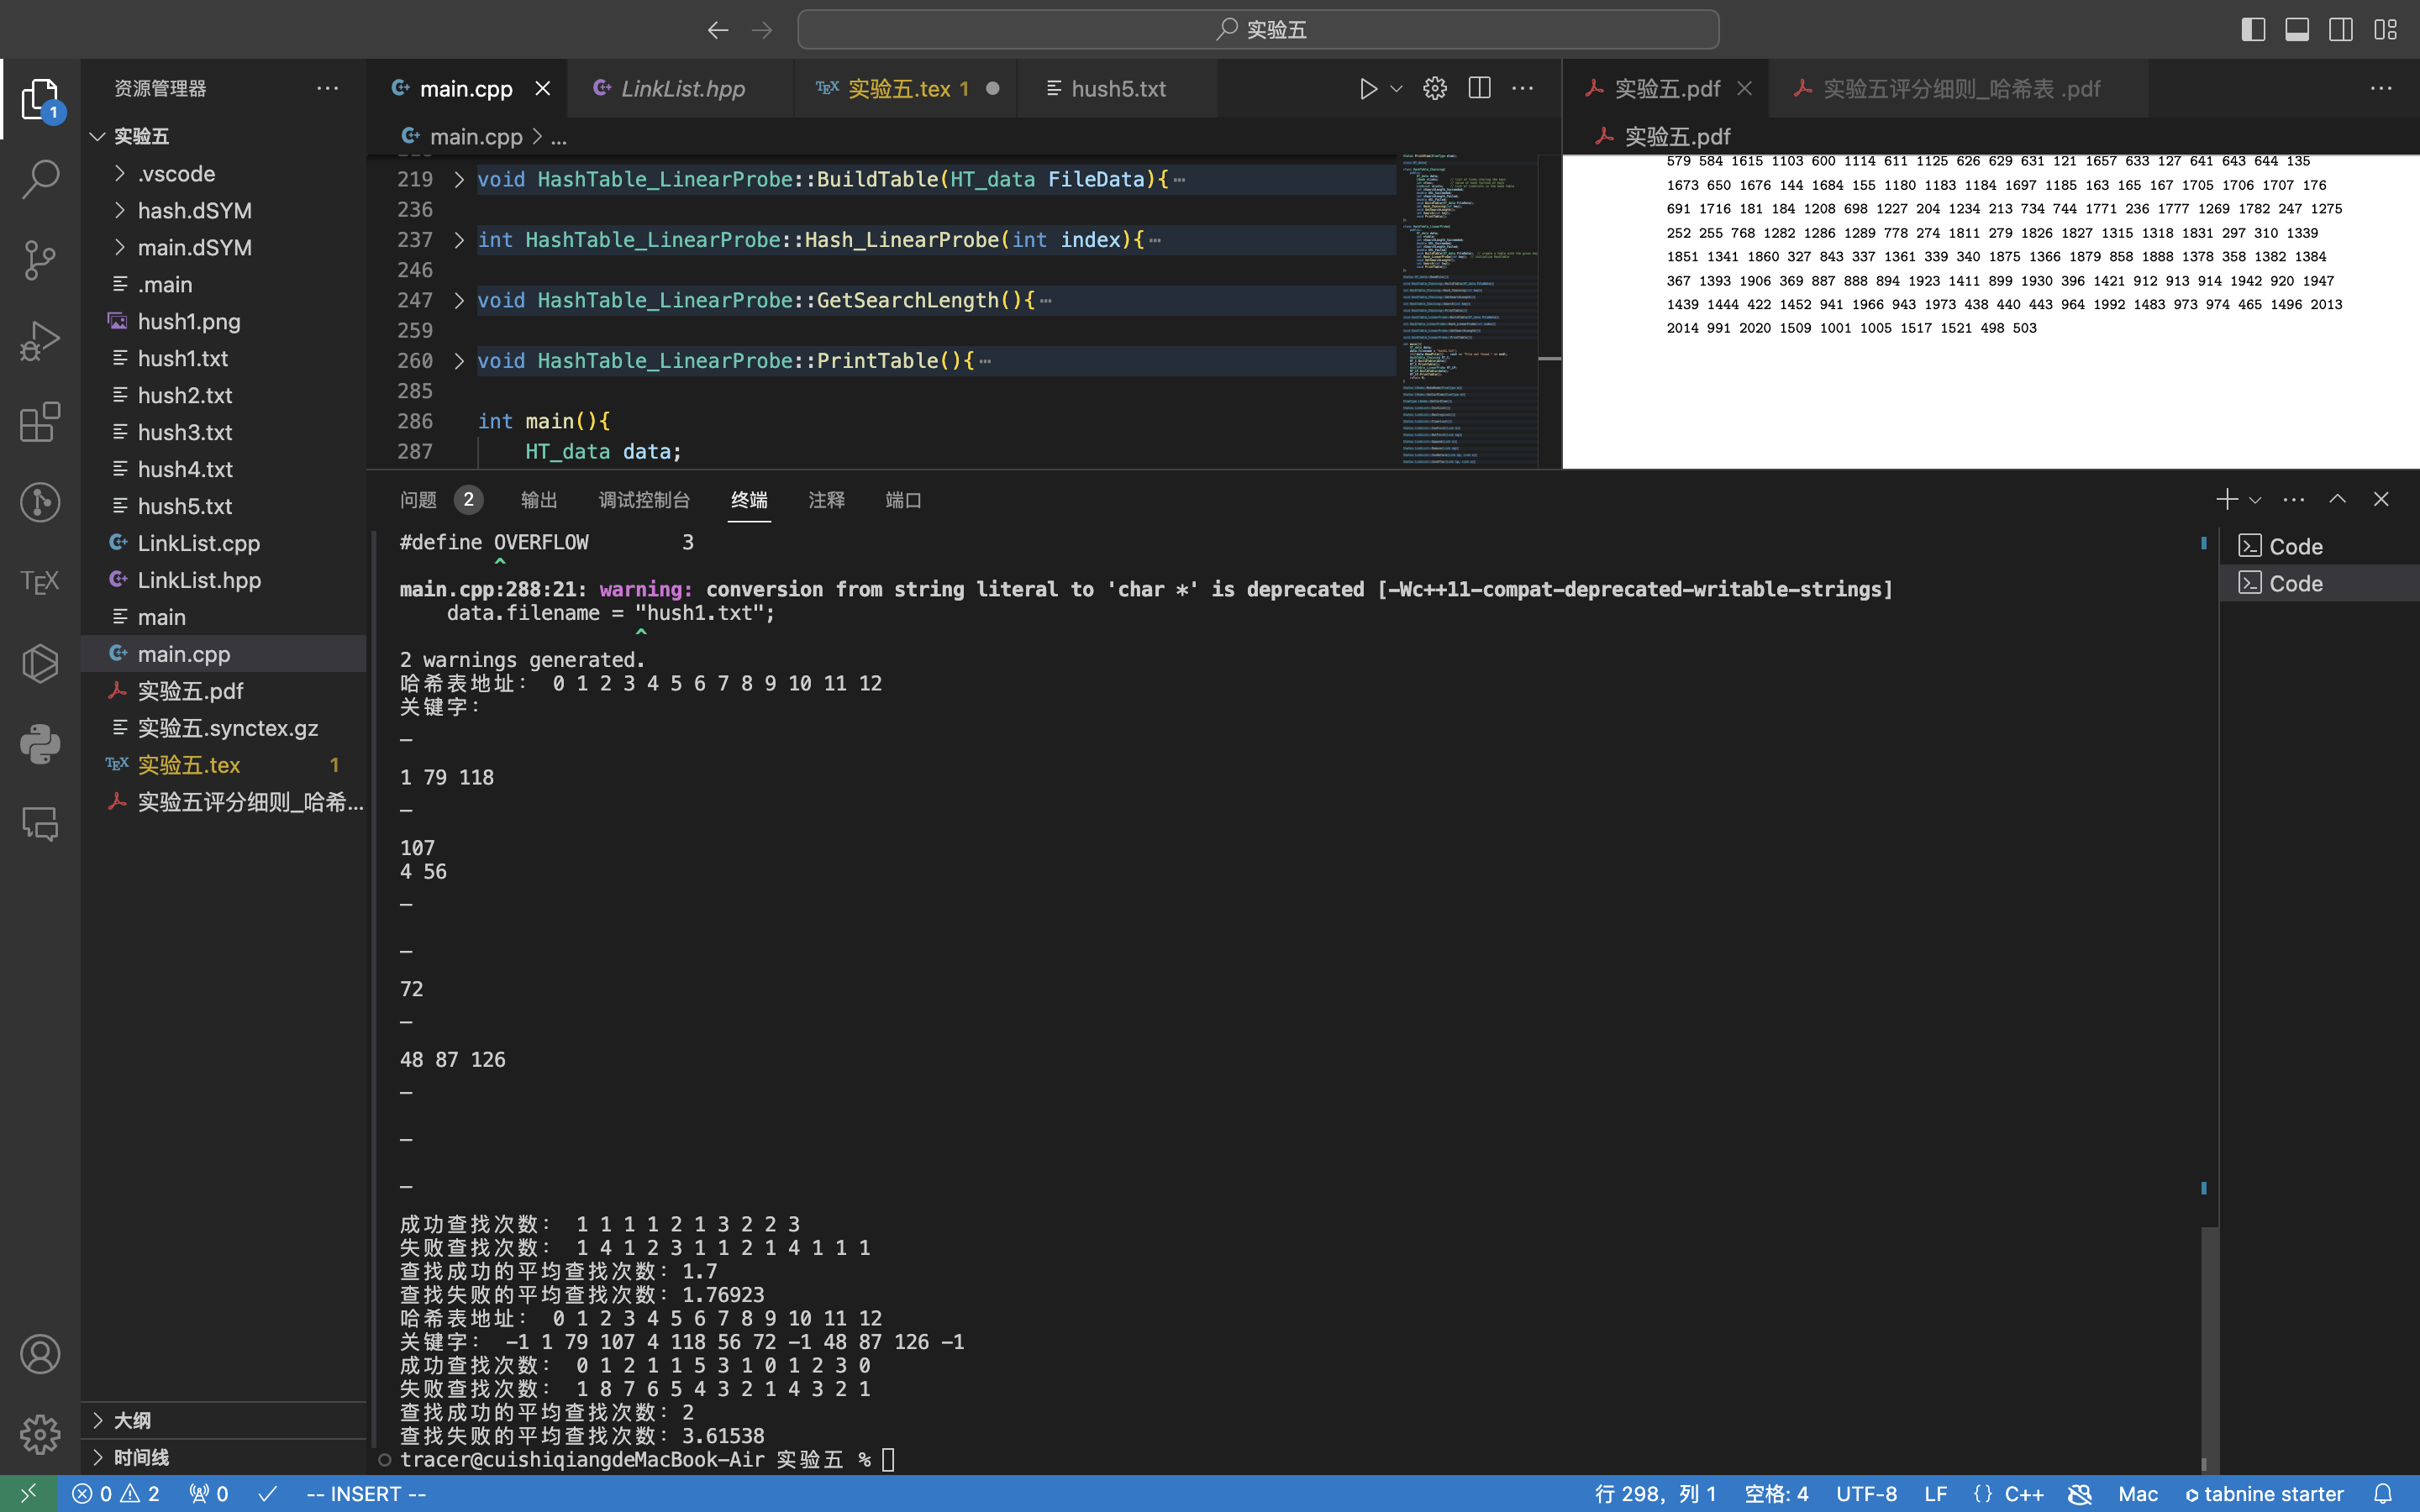
\includegraphics[scale=0.25]{hush1.png}
  \caption{hush1.txt}
\end{figure}
\begin{figure}[H]
  \centering
  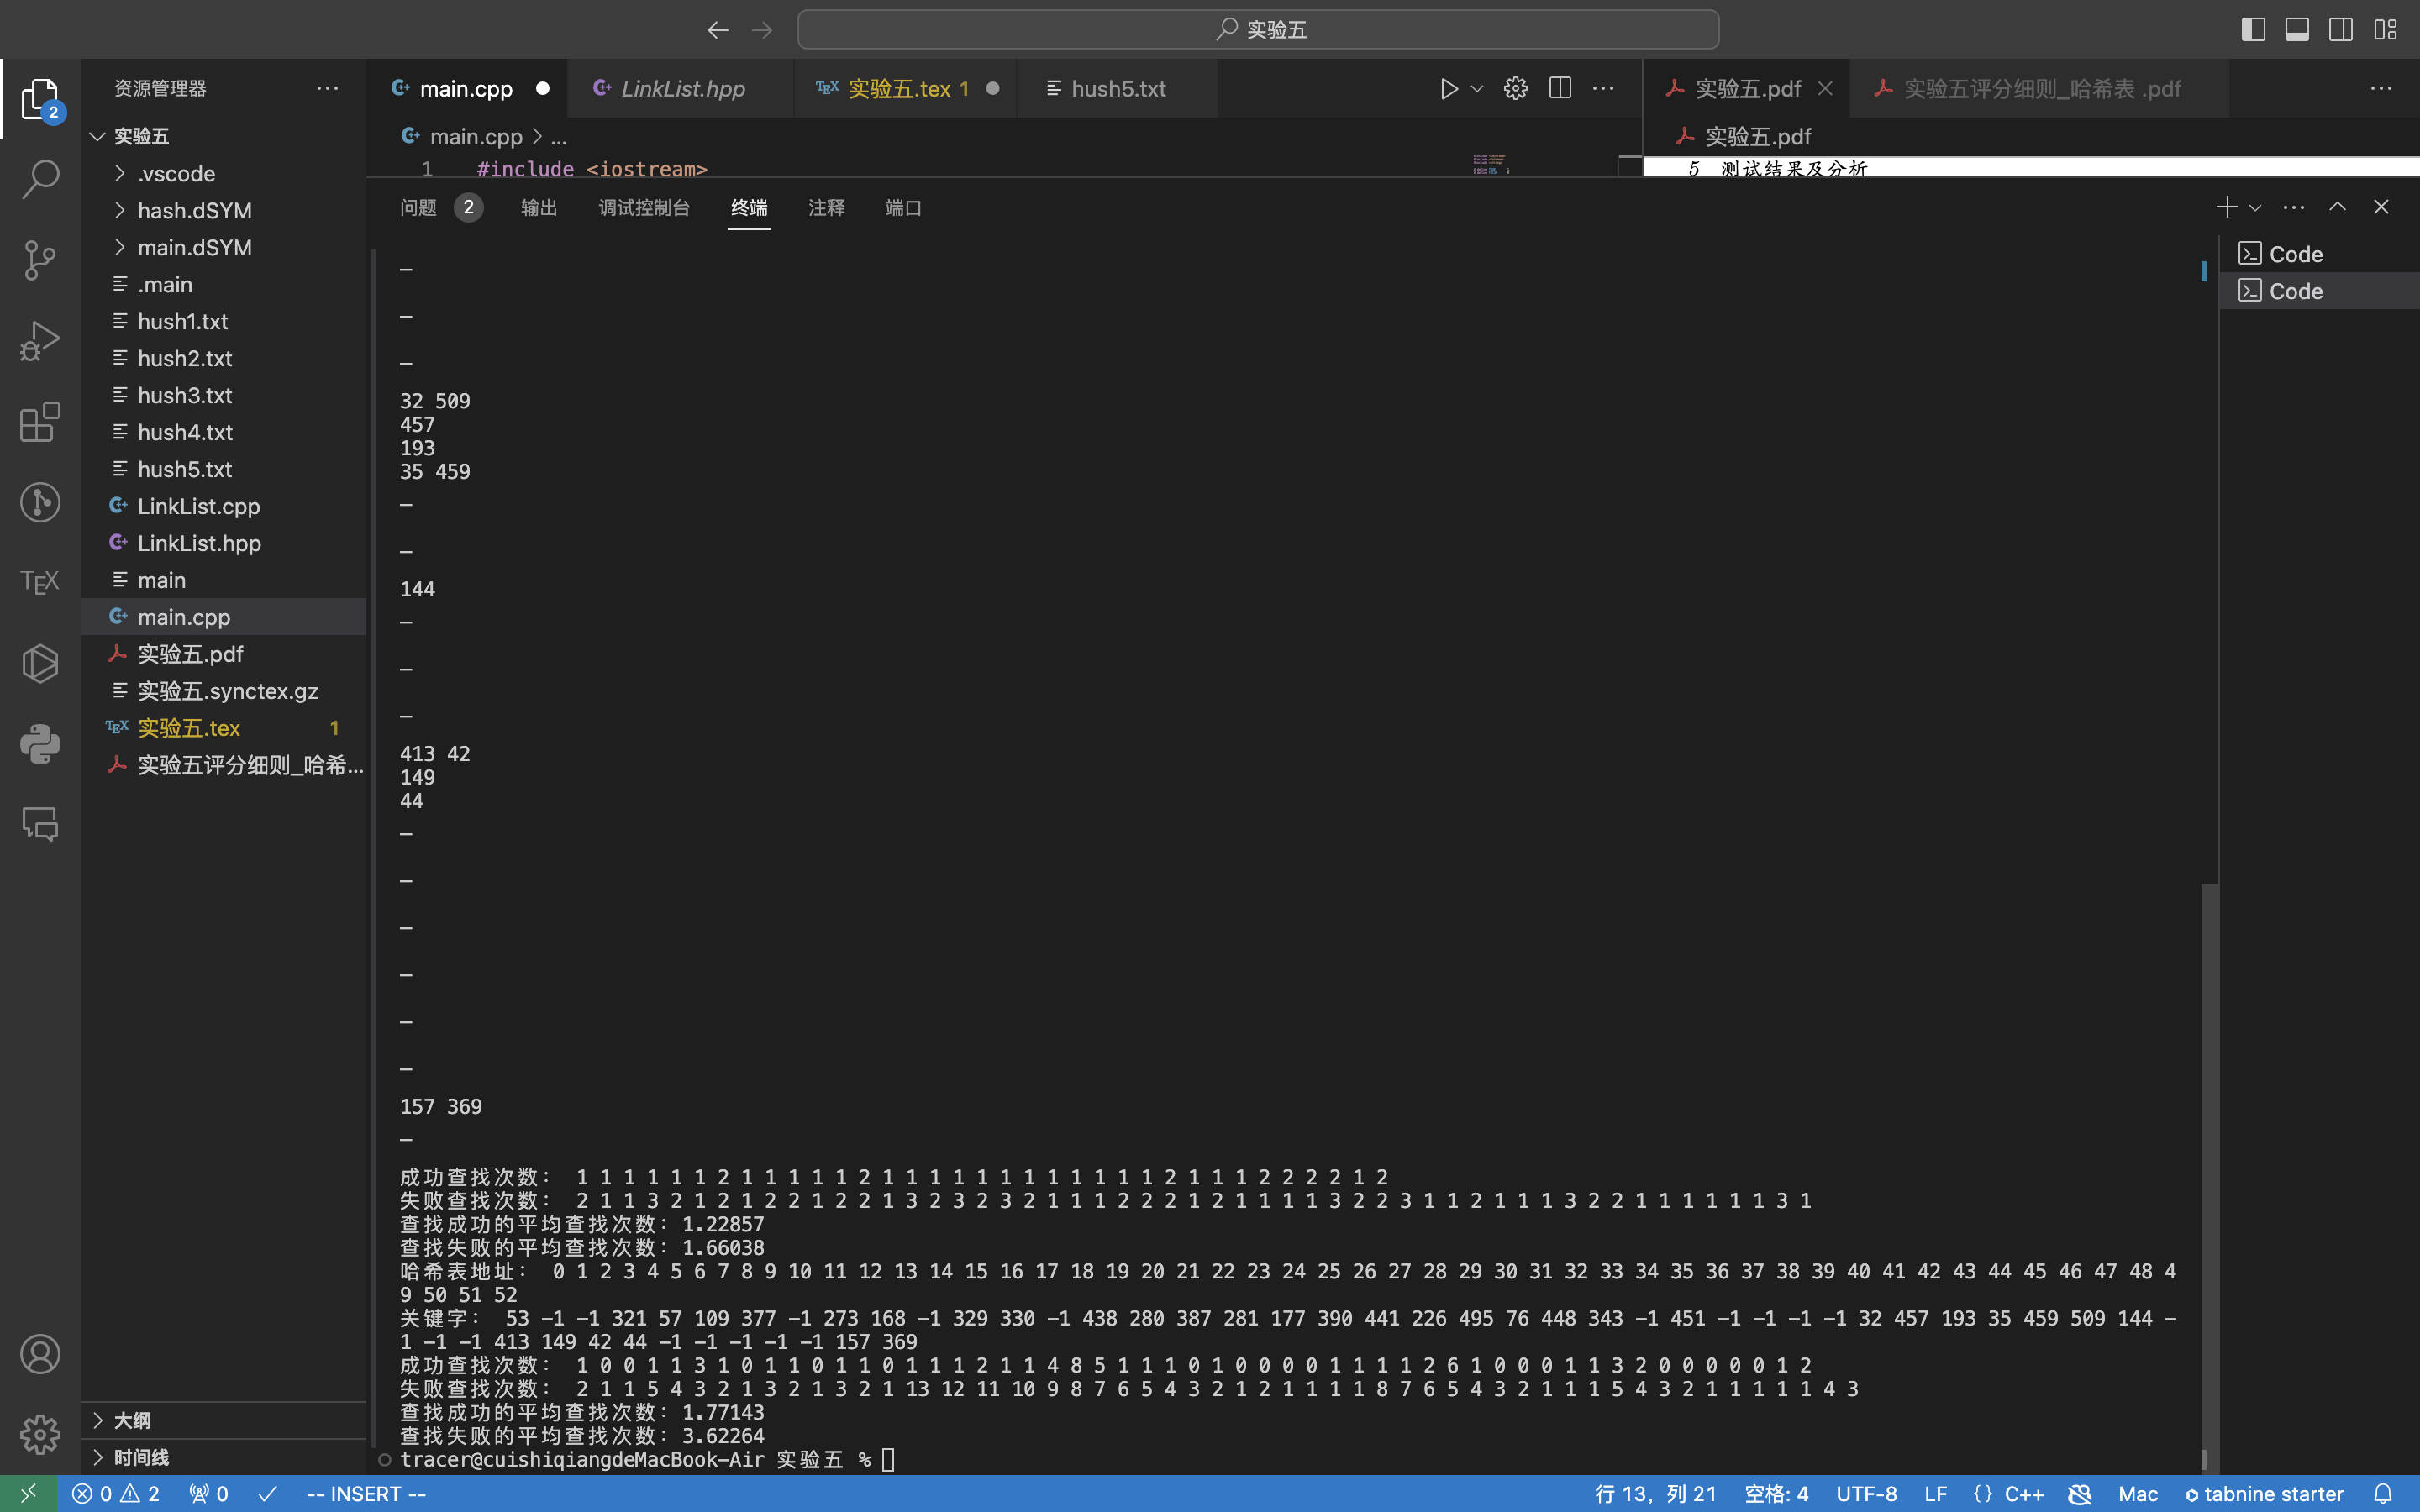
\includegraphics[scale=0.25]{hush2.png}
  \caption{hush2.txt}
\end{figure}
\begin{figure}[H]
  \centering
  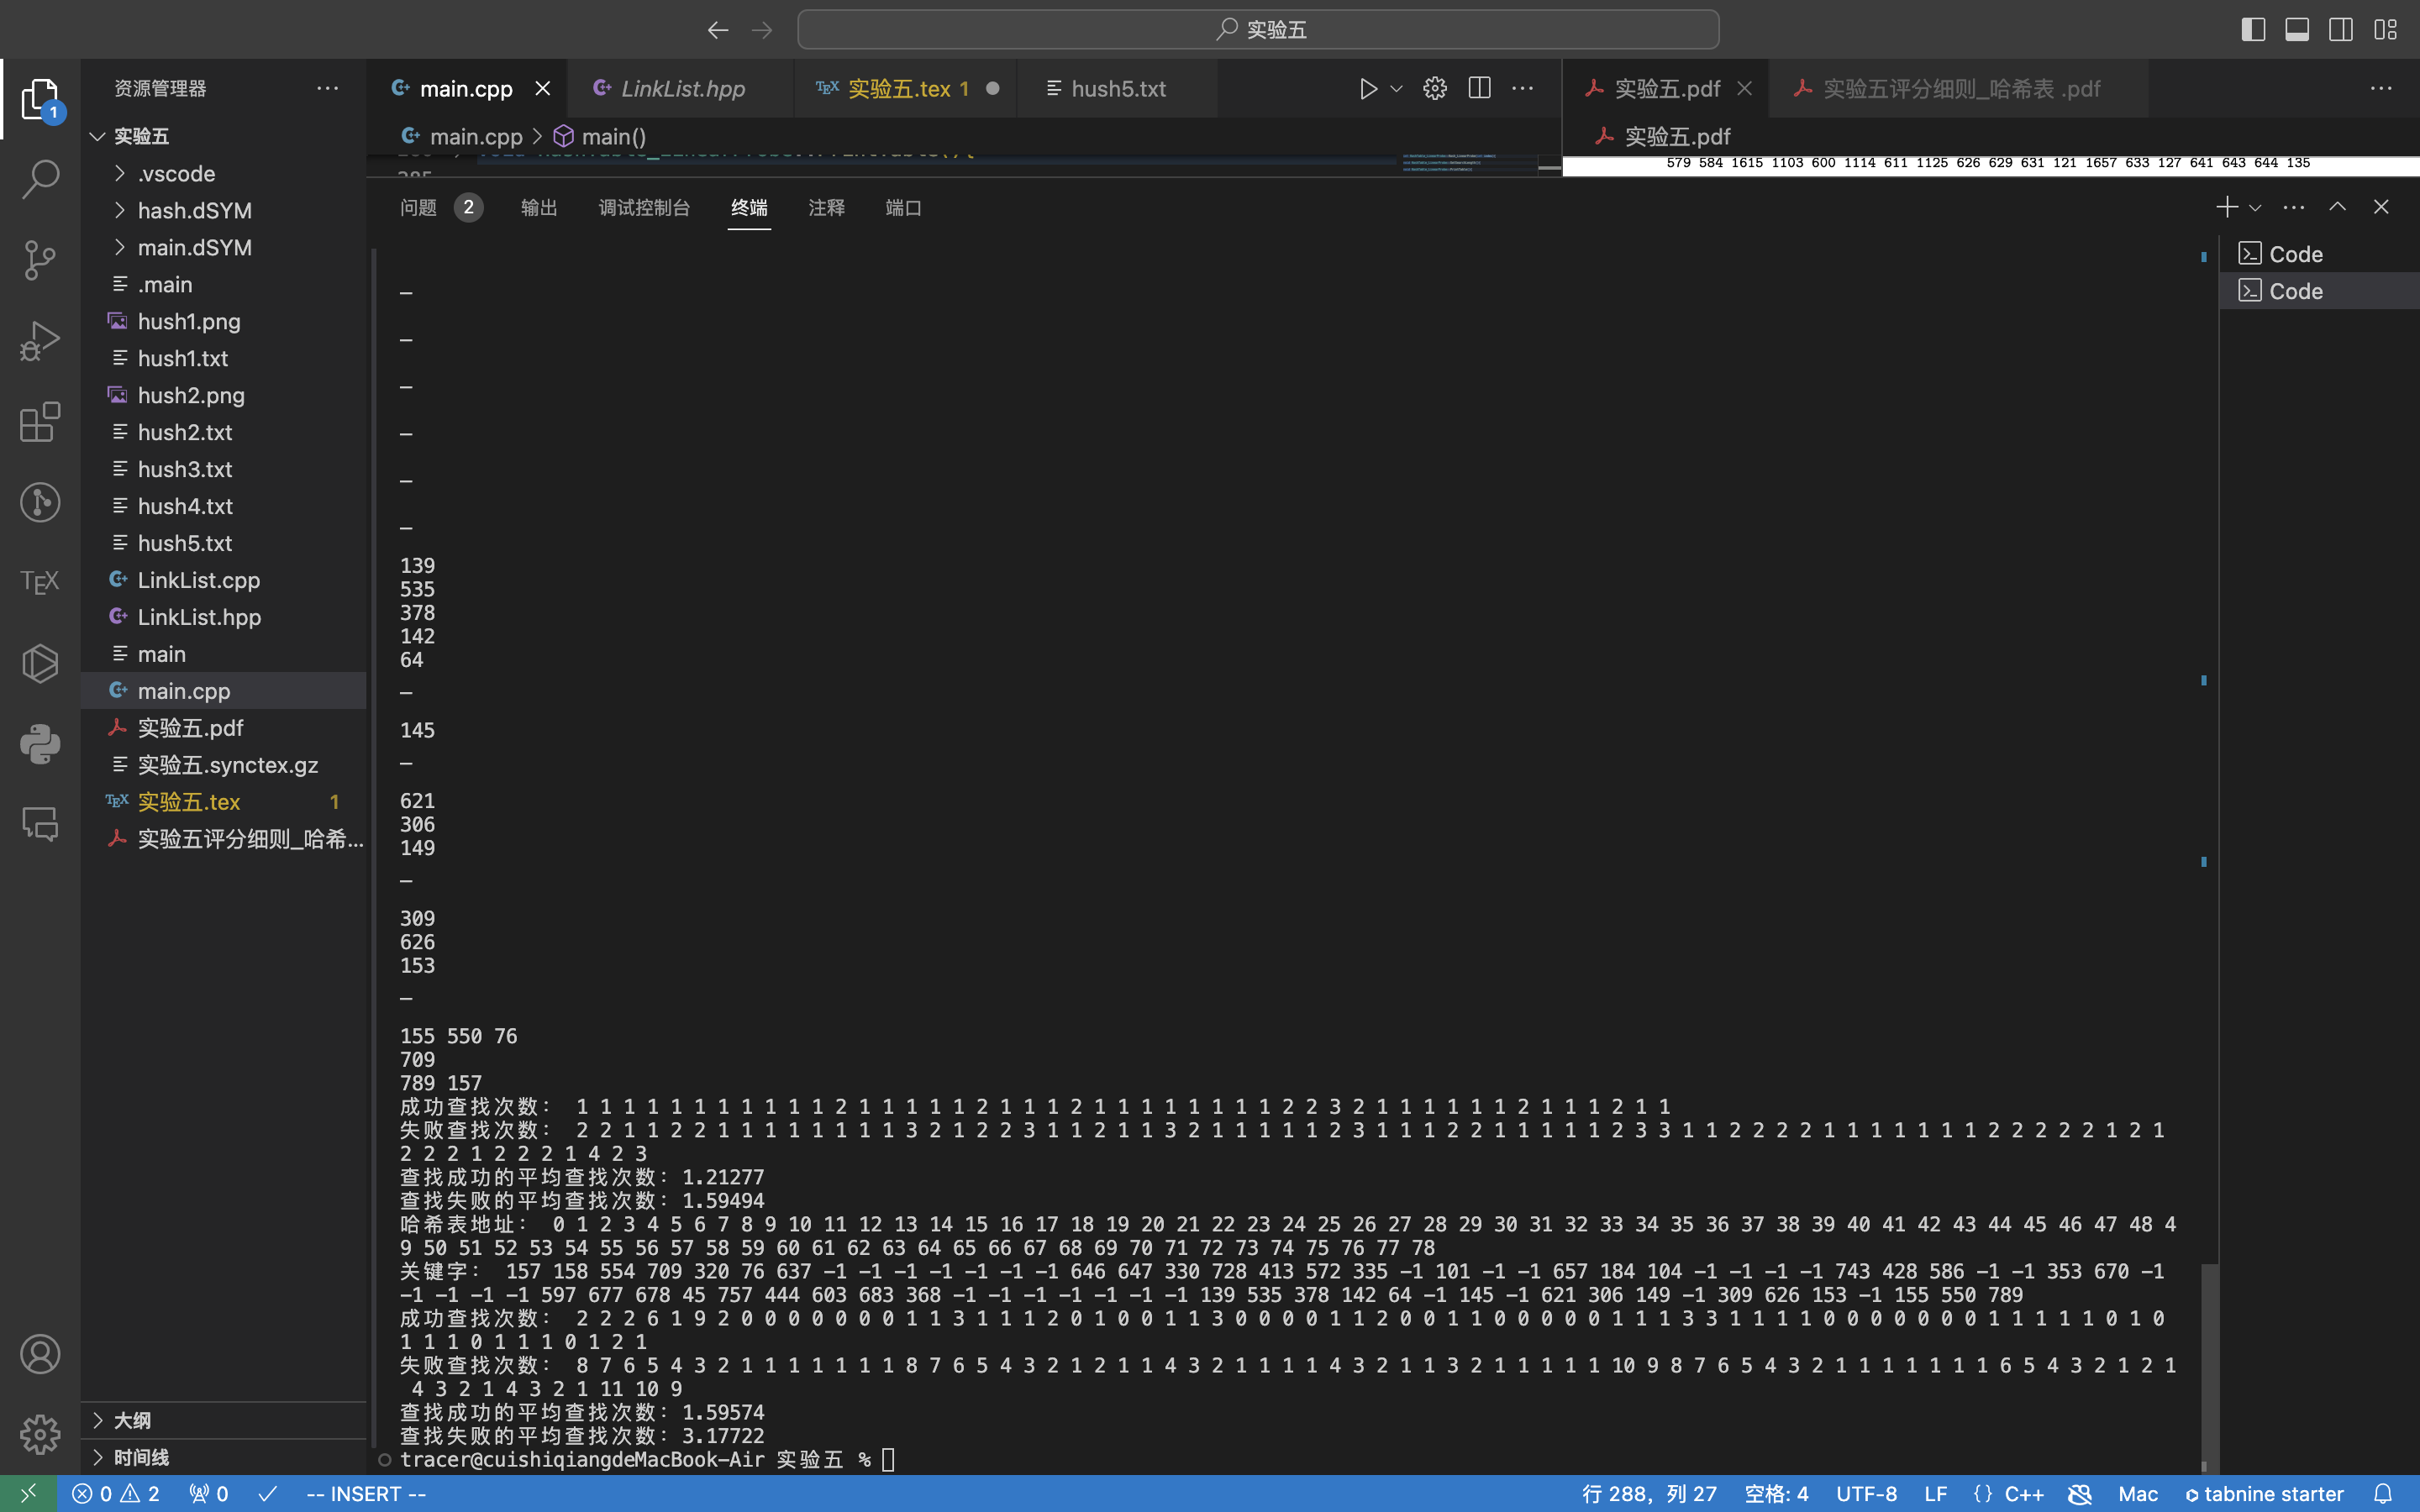
\includegraphics[scale=0.25]{hush3.png}
  \caption{hush3.txt}
\end{figure}
\begin{figure}[H]
  \centering
  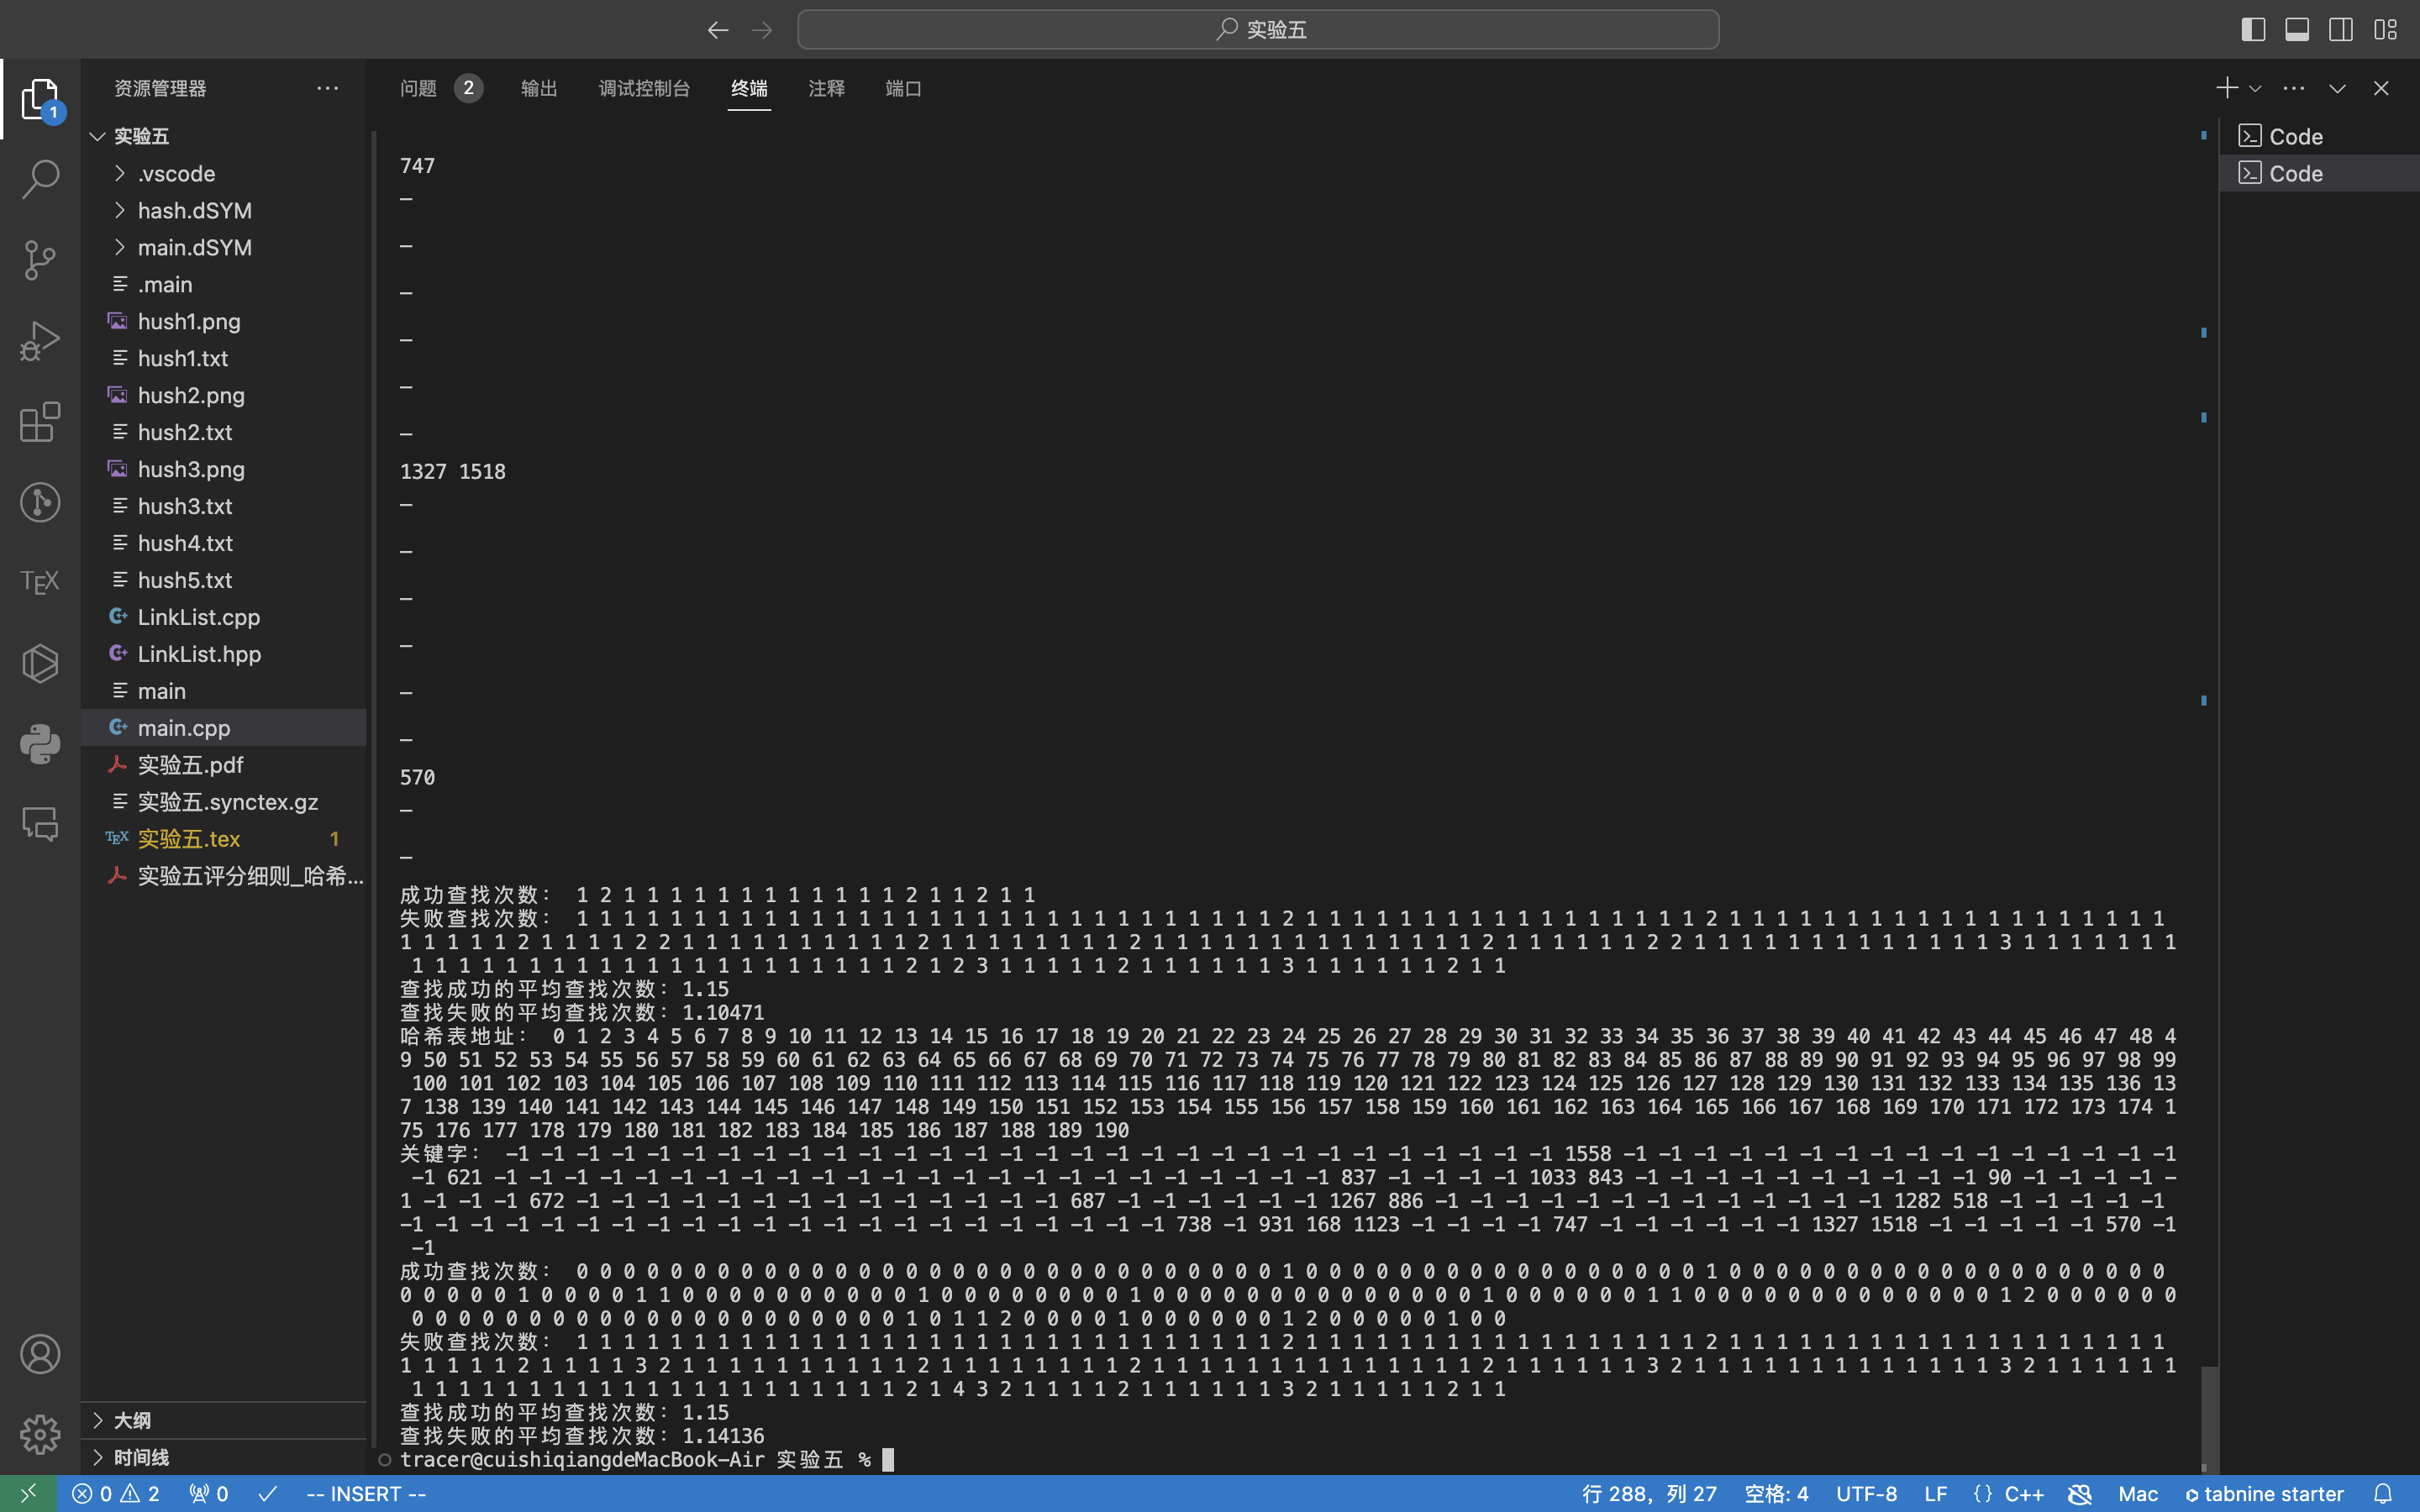
\includegraphics[scale=0.25]{hush4.png}
  \caption{hush4.txt}
\end{figure}
\begin{figure}[H]
  \centering
  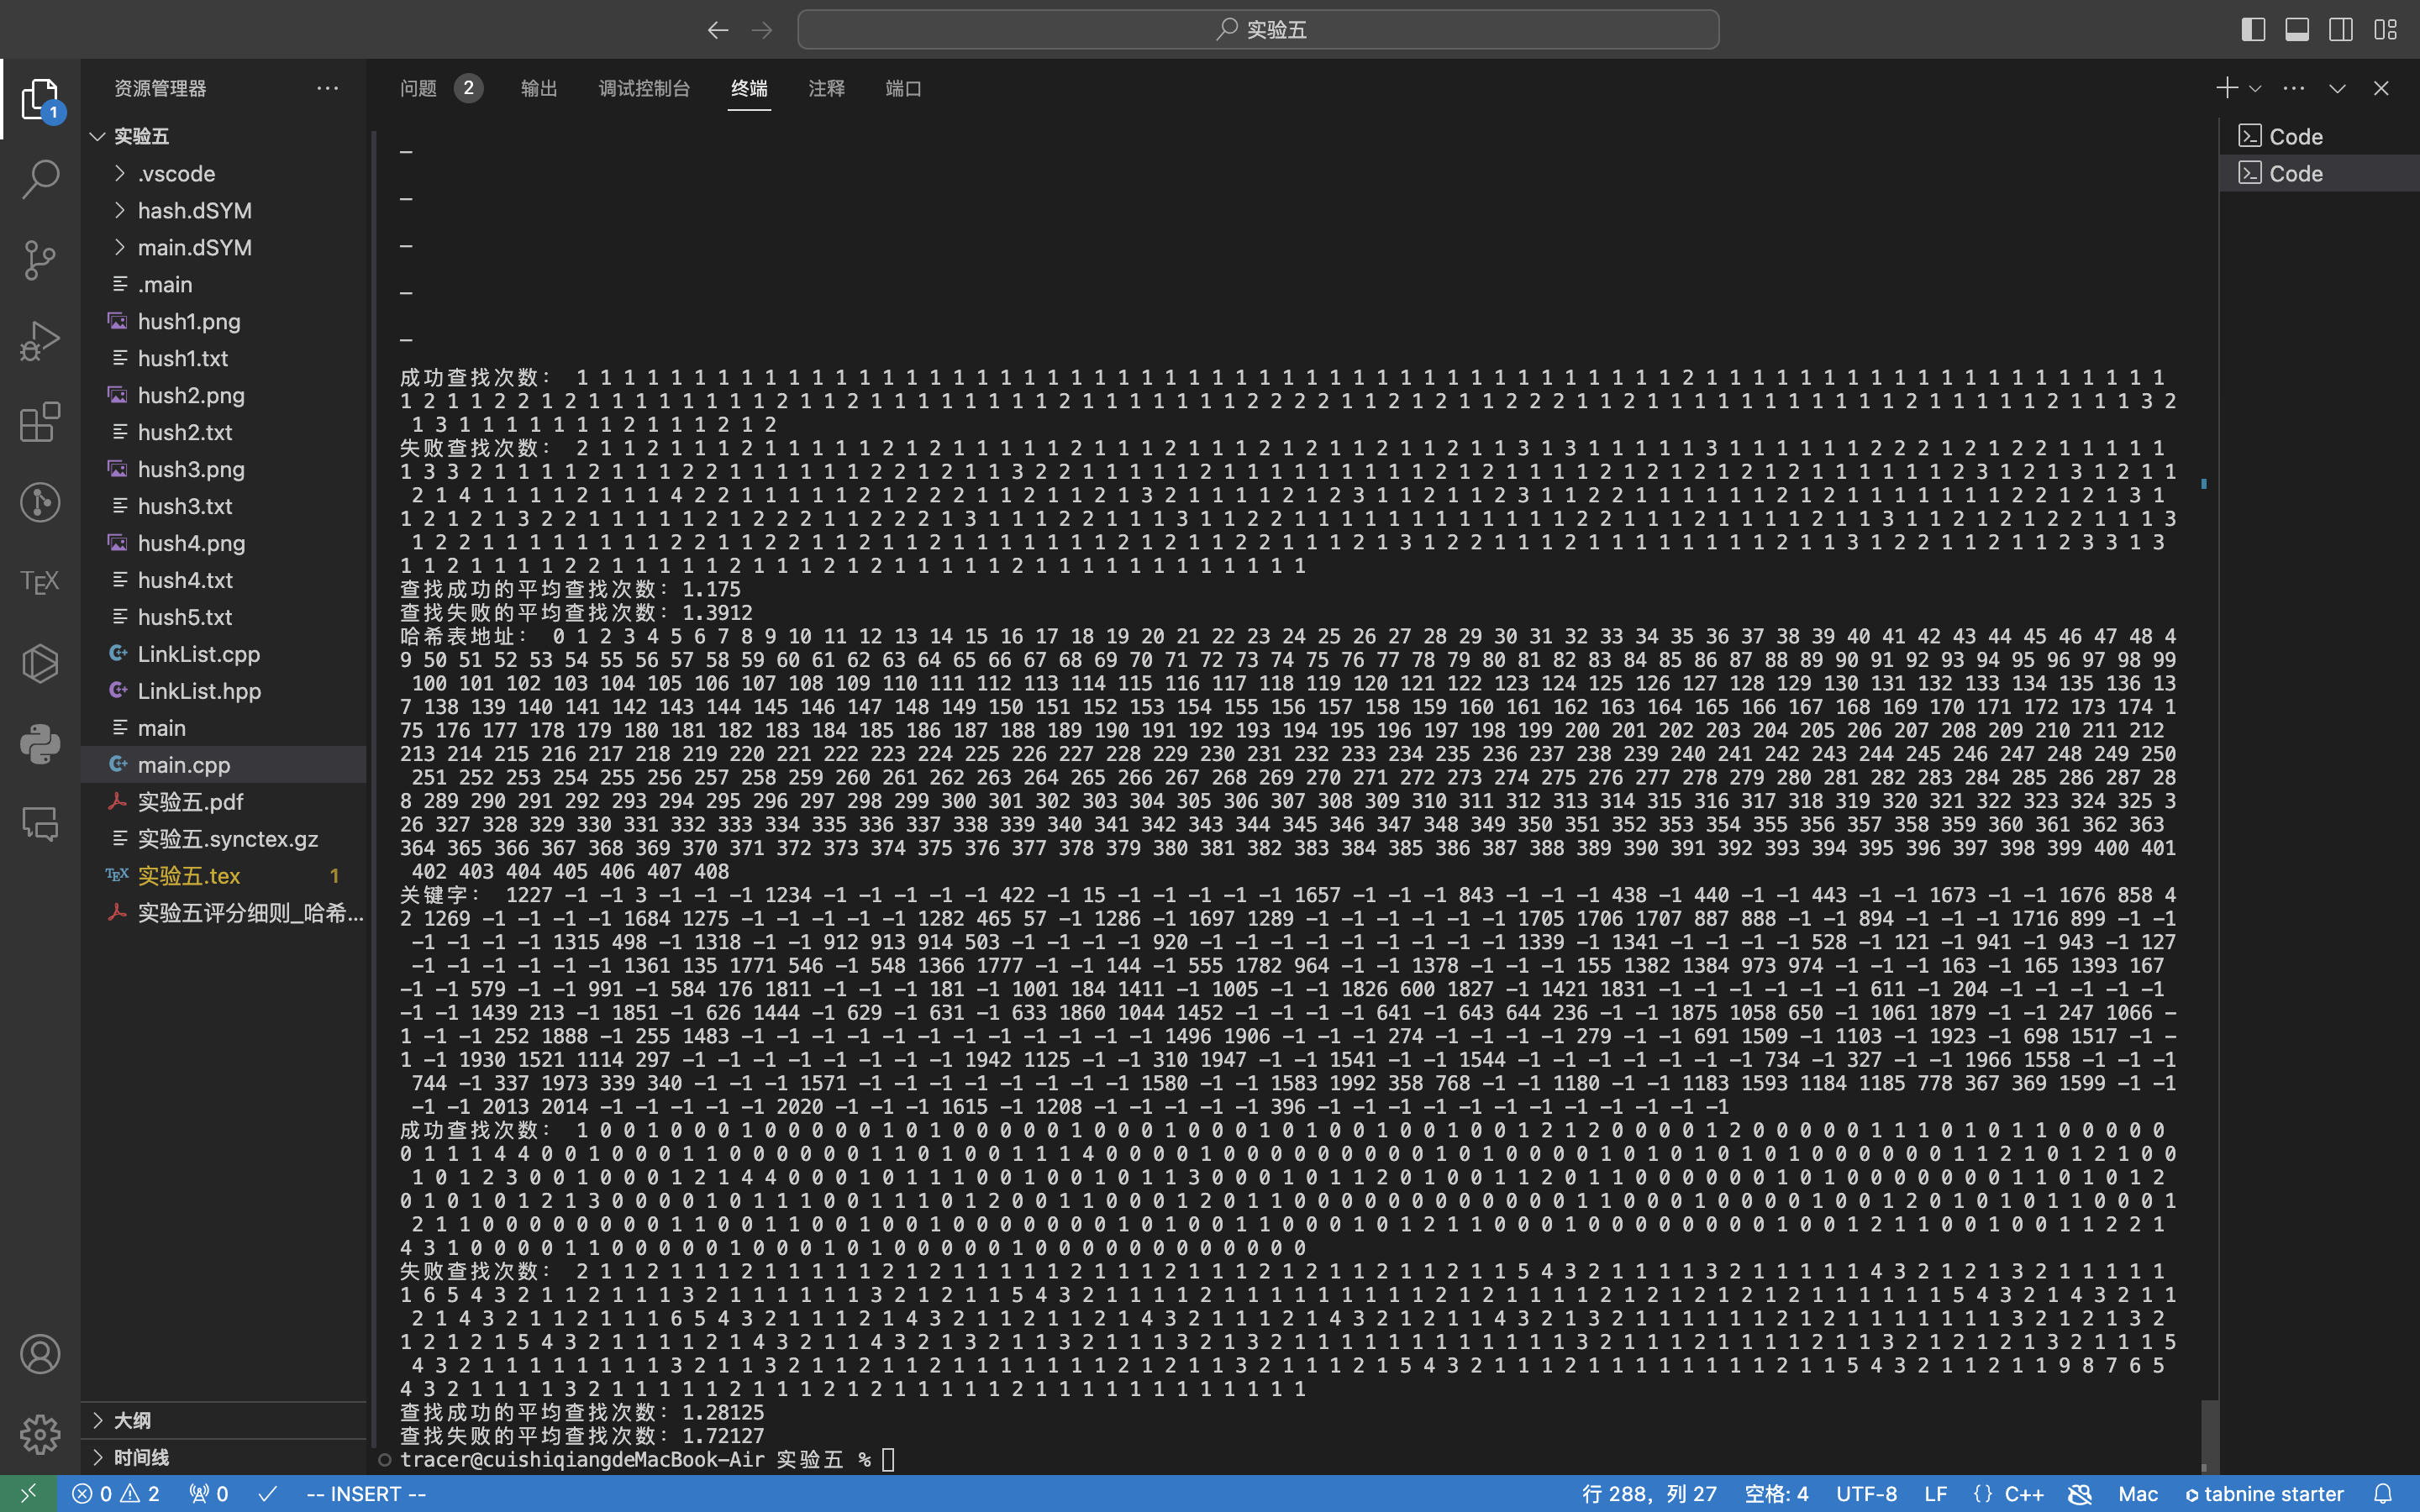
\includegraphics[scale=0.25]{hush5.png}
  \caption{hush5.txt}
\end{figure}
结果均正确.
\section{实验体会和收获}
通过实现两种构建哈希表的方法,理解了哈希表的原理、处理冲突的方式,掌握了存储以及快速查找数据的方法。
\end{document}
\iffalse
\begin{figure}[H]
    \centering
    \includegraphics[scale=0.5]{name.png}
    \caption{name}
\end{figure}
\fi
